\section{Αλγόριθμος Brushfire}
\label{section:brushfire_theory}

Ο αλγόριθμος \emph{Brushfire} ή \emph{Wavefront} είναι μια μέθοδος υπολογισμού  αποστάσεων μεταξύ σημείων σε έναν διακριτοποιημένο χώρο σε μορφή γράφου, όπως ένα OGM. Ο αλγόριθμος εκκινεί από ένα σύνολο σημείων του χώρου και βρίσκει τα αμέσως γειτονικά τους σημεία επαναληπτικά. Έτσι υπολογίζει την κοντινότερη απόσταση κάθε σημείου του ελεύθερου χώρου από το αρχικό υποσύνολο σημείων κρατώντας το πλήθος των επαναλήψεων που χρειάστηκαν για να φτάσει εως εκεί. Στην παρούσα διπλωματική η διαδικασία αυτή χρησιμοποιείται σε διάφορες παραλλαγές, ενώ σημειώνεται ότι σε όλες τις περιπτώσεις έχει υλοποιηθεί σε γλώσσα C για την βελτίωση της ταχύτητας της διαδικασίας των υπολογισμών. 

Επιπλέον, ως γειτονικά σημεία κάθε σημείου του χώρου μπορούν να θεωρηθούν είτε μόνο τα τέσσερα σημεία (βόριο, νότιο, ανατολικό και δυτικό) που παρουσιάζονται στο \autoref{fig:brushfire_neighbors_matrix} με πράσινο χρώμα είτε και τα οκτώ σημεία που βρίσκονται γύρω του. Στην μελέτη αυτή χρησιμοποιήθηκαν και τα 8 σημεία ως γείτονες σε όλες τις περιπτώσεις, καθώς έτσι προσεγγίζεται η πραγματική απόσταση μεταξύ σημείων με μεγαλύτερη ακρίβεια.

\begin{figure}[!htb]
    \centering
    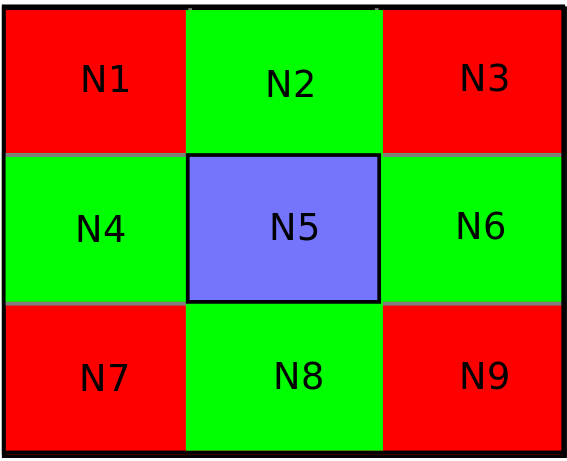
\includegraphics[width=0.3\textwidth]{./images/chapter3/neighbors2.png}
    \caption{Πίνακας γειτόνων σημείων}
    Πηγή: \href{http://roboscience.org/book/html/Planning/Brushfire.html}{http://roboscience.org/book/html/Planning/Brushfire.html}
    \label{fig:brushfire_neighbors_matrix}
\end{figure}
